\documentclass[conference]{IEEEtran}
\IEEEoverridecommandlockouts

\usepackage[T1]{fontenc}
\usepackage[utf8]{inputenc}
\usepackage{cite}
\usepackage{amsmath,amssymb,amsfonts}
\usepackage{graphicx}
\usepackage{booktabs}
\usepackage{array}
\usepackage{hyperref}
\usepackage{xcolor}
\usepackage{listings}
\usepackage{algorithm}
\usepackage{algpseudocode}
\usepackage{subcaption}
\usepackage{url}

\hypersetup{
    colorlinks=true,
    linkcolor=black,
    citecolor=black,
    urlcolor=blue
}

\lstdefinestyle{matlab}{
    language=Matlab,
    basicstyle=\ttfamily\footnotesize,
    numbers=left,
    numberstyle=\tiny,
    stepnumber=1,
    numbersep=6pt,
    breaklines=true,
    frame=single,
    columns=fullflexible,
    keepspaces=true
}

\newcommand{\acknowledgments}[1]{\textbf{Acknowledgments:} #1}

\begin{document}
\pagestyle{plain}

\title{Assignment 2: Lane Detection with GOLD Pipeline \\ Technologies for Autonomous Vehicles}

\author{
\IEEEauthorblockN{Anna Roma}
\IEEEauthorblockA{
\textit{Politecnico di Torino} \\
Student ID: 345819 \\
anna.roma@studenti.polito.it
}
}

\maketitle

\begin{abstract}
This report presents a MATLAB implementation of a lane detection pipeline inspired by the GOLD algorithm and designed for real road images from the PandaSet front camera. The method combines inverse perspective mapping, region-of-interest masking, image enhancement, adaptive thresholding, histogram-based lane initialization and lane tracking in Bird's Eye View. The system detects the left and right lane delimiters, distinguishes between solid and dashed markings, visualizes the final output on the original image, and integrates obstacle detection with approximate distance estimation. The experimental results show that the proposed pipeline is able to robustly detect both straight and curved lane markings and to integrate obstacle detection within the lane.
\end{abstract}

\section{Introduction}
Lane detection is a core perception task for advanced driver assistance systems and autonomous vehicles. Reliable detection of lane delimiters supports lateral localization, lane keeping, path planning and safety monitoring. In practice, however, the problem is challenging because road images are affected by perspective distortion, varying illumination, shadows, worn lane markings, occlusions and traffic participants.

The goal of this assignment is to implement a lane detection algorithm that processes each image in a given PandaSet directory and produces a visualization of the detected lane delimiters. The assignment also includes three optional extensions: discrimination between solid and dashed lane markings, visualization on the original image instead of the Bird's Eye View (BEV), and obstacle recognition with approximate distance estimation.

The solution developed in this work follows the spirit of the GOLD algorithm proposed by Bertozzi and Broggi \cite{gold_paper}. The key idea is to transform the input image into a top-down representation of the road, where lane markings become easier to analyze. On top of this classical vision pipeline, an object detector is integrated to identify road users and highlight obstacles located inside the lane.

\section{Background}
\subsection{The GOLD approach}
The GOLD algorithm is a classical vision-based framework for generic obstacle and lane detection \cite{gold_paper}. Its main strength is the use of a geometric transformation that removes most of the perspective effect from the road image. Once the scene is mapped to a BEV representation, lane delimiters are approximately vertical and their localization can be simplified through intensity analysis and geometric constraints.

Even though the original GOLD system was designed for real-time stereo vision, several of its core ideas remain highly relevant in monocular lane detection:
\begin{itemize}
    \item restriction of the analysis to the road region;
    \item inverse perspective mapping to simplify geometry;
    \item enhancement of bright lane markings against darker asphalt;
    \item lane localization through compact features rather than dense segmentation.
\end{itemize}

These principles are directly reflected in the implemented pipeline.

\subsection{Object detection}

To extend the perception capability beyond lane detection, the proposed system also includes an object-detection module. When available, the implementation employs YOLO (You Only Look Once) \cite{yolo}, a one-stage object detector that simultaneously predicts bounding boxes, class labels, and confidence scores in a single forward pass.

In this work, the preferred detector is a pretrained \texttt{YOLOv4-tiny} model provided by MATLAB (\texttt{yolov4ObjectDetector("tiny-yolov4-coco")}). The network is trained on the COCO dataset and is adopted directly for inference, without performing any additional training or fine-tuning on the PandaSet data. If the YOLO support package is not available, the code falls back to MATLAB ACF-based vehicle and pedestrian detectors, so that obstacle detection remains available.

The detector operates on the original RGB image, independently of the lane detection pipeline. The raw detections are then filtered by:
\begin{itemize}
    \item selecting only relevant classes (e.g., cars, trucks, buses, bicycles, motorcycles, and pedestrians);
    \item discarding detections outside the road Region of Interest (ROI).
\end{itemize}

Finally, the remaining bounding boxes are geometrically compared with the detected lane boundaries in order to determine whether an obstacle lies within the current driving lane. This integration allows combining object detection with the classical vision-based lane estimation, improving the overall robustness of the system.

\section{Problem Formulation}
Given an RGB image acquired by the PandaSet front camera, the objective is to estimate the visible left and right lane delimiters and produce an interpretable visualization for every frame in the input directory. More formally, the algorithm must:
\begin{enumerate}
    \item process all the images addressed by the variable \texttt{search\_path};
    \item identify the lane boundaries, when visible, within the road portion of the image;
    \item display the detected lane delimiters and the message \textit{No lanes found} when neither lane is available;
    \item optionally classify each lane delimiter as solid or dashed;
    \item optionally visualize the lanes on the original image;
    \item optionally identify obstacles in the lane and report an approximate distance.
\end{enumerate}

The implementation assumes a flat-road approximation in the BEV transformation and exploits the calibrated monocular camera parameters provided in the assignment text.

\section{Dataset and Camera Model}
The algorithm is designed for the PandaSet front camera images specified in the assignment. The supplied camera parameters are used to instantiate the MATLAB monocular camera model and to build the inverse perspective mapping used throughout the pipeline.

\begin{table}[htbp]
\caption{Camera parameters used in the implementation}
\label{tab:camera}
\centering
\begin{tabular}{ll}
\toprule
Parameter & Value \\
\midrule
Image size & $1920 \times 1080$ px \\
Principal point & $(970,\ 483)$ px \\
Focal length & $(1970,\ 1970)$ px \\
Camera position & $(1.875,\ 0,\ 1.660)$ m \\
Camera pitch & $0^\circ$ \\
\bottomrule
\end{tabular}
\end{table}

The camera model is instantiated in MATLAB through \texttt{cameraIntrinsics} and \texttt{monoCamera}. A \texttt{birdsEyeView} object is then defined over a road patch extending from 5 m to 40 m ahead of the vehicle and spanning 5 m to both the left and right of the ego lane.

\section{Methodology}
\subsection{Pipeline}
The complete processing chain is summarized below:
\begin{enumerate}
    \item image loading from \texttt{search\_path};
    \item camera-based transformation to BEV;
    \item trapezoidal ROI definition and projection into BEV;
    \item grayscale conversion and Gaussian smoothing;
    \item lane enhancement via morphological top-hat filtering;
    \item adaptive binarization with separate thresholds for the left and right halves of the image;
    \item histogram-based initialization of lane positions;
    \item row-wise lane tracing in BEV to follow straight and moderately curved markings;
    \item classification of the detected lanes as solid or dashed;
    \item object detection on the original image;
    \item lane-aware obstacle filtering and approximate distance estimation;
    \item visualization and result export.
\end{enumerate}

\subsection{Region of interest}
The first robustness measure is the definition of a trapezoidal ROI in the original image. This mask removes irrelevant content such as sky, buildings and roadside clutter, concentrating the analysis on the road surface. The trapezoid is centered around the optical axis and widened toward the bottom of the image, coherently with the camera perspective.

After defining the ROI in image coordinates, the polygon is projected into the vehicle frame and then mapped to the BEV image. This produces a binary mask that is reused throughout the pipeline to keep only the pixels that belong to the road region.

\subsection{Bird's Eye View transformation}
Perspective projection makes lane localization difficult because the same physical lane width occupies different image widths depending on the distance from the camera. To reduce this effect, the image is remapped to a Bird's Eye View using the road-plane assumption.

In the BEV domain, lane delimiters become approximately vertical and their lateral position can be studied with simpler image statistics. This representation is central to the whole method because it enables both histogram-based initialization and row-wise lane tracing.

\subsection{Image preprocessing and lane enhancement}
Once the BEV image is available, it is converted to grayscale:
\begin{equation}
I_g = \mathrm{rgb2gray}(I_{\text{BEV}}).
\end{equation}

The grayscale image is then smoothed with a Gaussian filter to reduce high-frequency noise:
\begin{equation}
I_f = G_\sigma * I_g,
\end{equation}
where $G_\sigma$ is a Gaussian kernel with standard deviation selected empirically in the implementation.

To enhance lane markings, a morphological top-hat operator is applied using a vertical structuring element. This operation emphasizes bright elongated structures against the darker road background:
\begin{equation}
I_e = I_f - (I_f \circ b),
\end{equation}
where $\circ$ denotes morphological opening and $b$ is the chosen structuring element.

\subsection{Adaptive thresholding with left-right split}
Because the road appearance may differ between the left and right halves of the image due to illumination, shadows or worn paint, a single global threshold may be unstable. For this reason, the BEV image is split into two halves and an iterative threshold is computed independently on each side.

Let $P$ be the set of valid pixels inside the masked region of one half-image. Starting from
\begin{equation}
T^{(0)} = \frac{\max(P) + \min(P)}{2},
\end{equation}
the pixels are iteratively separated into two groups above and below the current threshold. If $\mu_A$ and $\mu_B$ are the corresponding group means, the threshold is updated as
\begin{equation}
T^{(k+1)} = \frac{\mu_A + \mu_B}{2}.
\end{equation}
The process stops when the threshold variation becomes negligible. The final binary lane map is obtained by combining the left and right thresholded halves. This design follows the suggestion given during the course and improves robustness under asymmetric lighting conditions.

\subsection{Lane initialization through histogram analysis}
After binarization and removal of small connected components, the algorithm computes a column-wise histogram over the lower half of the BEV image. Since lane delimiters appear approximately vertical, the column sum produces peaks close to the horizontal positions of the lane markings.

The histogram is split into left and right regions. The strongest peak in each half is used as an initial estimate for the corresponding lane. Minimum peak height and minimum peak distance constraints reduce false positives.

\subsection{Lane tracing and handling of curved roads}
Using only a single vertical line for visualization is insufficient, especially when the road is curved. For this reason, the final implementation traces each lane row by row in the BEV image.

Starting from the initial peak location, the algorithm scans the binary BEV from bottom to top. At each row, it searches for active lane pixels in a horizontal window around the previous position. If multiple pixel groups are found, the group center closest to the previous estimate is selected. In this way, the lane position can evolve with the road geometry rather than remaining fixed at a single column.

This row-wise strategy is important for two reasons:
\begin{itemize}
    \item it provides a more realistic lane shape in the visualization;
    \item it improves behavior on roads that are not perfectly straight, including moderate curves.
\end{itemize}

\subsection{Solid versus dashed lane classification}
The optional requirement on lane-type discrimination is addressed by analyzing the continuity of the traced lane support. Once a lane has been tracked in BEV, the algorithm evaluates how many rows contain valid lane evidence in the analyzed lower portion of the image.

A solid lane generally produces a long and continuous response, while a dashed lane generates separated visible segments with missing intervals. This difference is captured by the support mask of the traced lane, which is then compared with empirically chosen thresholds to assign the label \texttt{solid} or \texttt{dashed}.

Moreover, the visualization preserves the lane morphology: solid lanes are rendered as continuous curves, while dashed lanes are displayed with interruptions matching the detected support.

\subsection{Temporal robustness through short-term memory}
Real driving frames may temporarily miss one or both lane markings because of occlusions, worn paint or abrupt lighting changes. To reduce visual flicker and improve robustness, the implementation stores the most recent valid lane detections for a limited number of frames.

If the current image does not provide a valid lane estimate, the system reuses the last reliable detections within a short temporal window. This mechanism does not replace the current estimate when a new valid detection is available; it only acts as a fallback during brief failures.

\subsection{Obstacle detection and distance estimation}
The object detector is executed on every original image. The detected objects are filtered in two steps. First, only relevant road users are kept. Second, the lower support points of each bounding box are tested against the trapezoidal road ROI so that detections outside the road region are discarded while preserving distant objects whose box center may lie above the ROI.

For each retained obstacle, an approximate distance is estimated from the image-space bounding-box height:
\begin{equation}
d \approx \frac{H f_y}{h_{\text{bbox}}},
\end{equation}
where $H$ is a nominal real-world object height, $f_y$ is the vertical focal length and $h_{\text{bbox}}$ is the bounding-box height in pixels. This approximation is simple and not category-specific, but it is sufficient to provide an indicative distance value for the assignment.

To determine whether an obstacle is inside the current lane, the bottom center of the bounding box is projected into the BEV domain and compared with the interpolated left and right lane boundaries at the same longitudinal position. If the projected point falls between the two lane delimiters, the obstacle is marked as being in-lane.

\subsection{Visualization Strategy}
The assignment requires the visualization of detected lanes, optionally directly on the original image. This requirement is fulfilled by projecting the lane points extracted in the Bird’s Eye View (BEV) back onto the original camera frame and overlaying them on the RGB image.
For each processed frame, a multi-panel visualization is generated, including: the original image with ROI, lane detections, and obstacle detections; the grayscale BEV with detected lanes; the ROI mask; the enhanced BEV image; the binary BEV image; and the column histogram used for lane initialization.
To enhance robustness against occasional detection failures, a temporal consistency mechanism is introduced. In cases where a lane is not detected in the current frame, the system retains and displays the last valid detection for up to five consecutive frames. This strategy mitigates visual instability and reduces flickering effects.
The proposed visualization scheme supports both qualitative evaluation and effective debugging of the intermediate stages of the pipeline.


\section{Implementation Notes}
The full solution is implemented in MATLAB in the file \texttt{main.m}. The input image directory is specified through the variable \texttt{search\_path}; however, the user must provide the correct local path to the dataset archive, since it is not included in the project folder due to its large size (due to GitHub limitations). The script iterates over every image in the selected directory, processes it independently, and saves the generated visualizations in the \texttt{results} folder.

\section{Results}
The algorithm was evaluated qualitatively on five different PandaSet scenarios, selected to include straight roads, curved dashed markings, close obstacles, distant road users and partial occlusions. The generated output for each frame contains both the final overlay on the original image and the intermediate BEV processing stages, making it possible to inspect not only the final detection but also the behavior of the ROI mask, the binary image and the column histogram.

\begin{figure}[htbp]
    \centering
    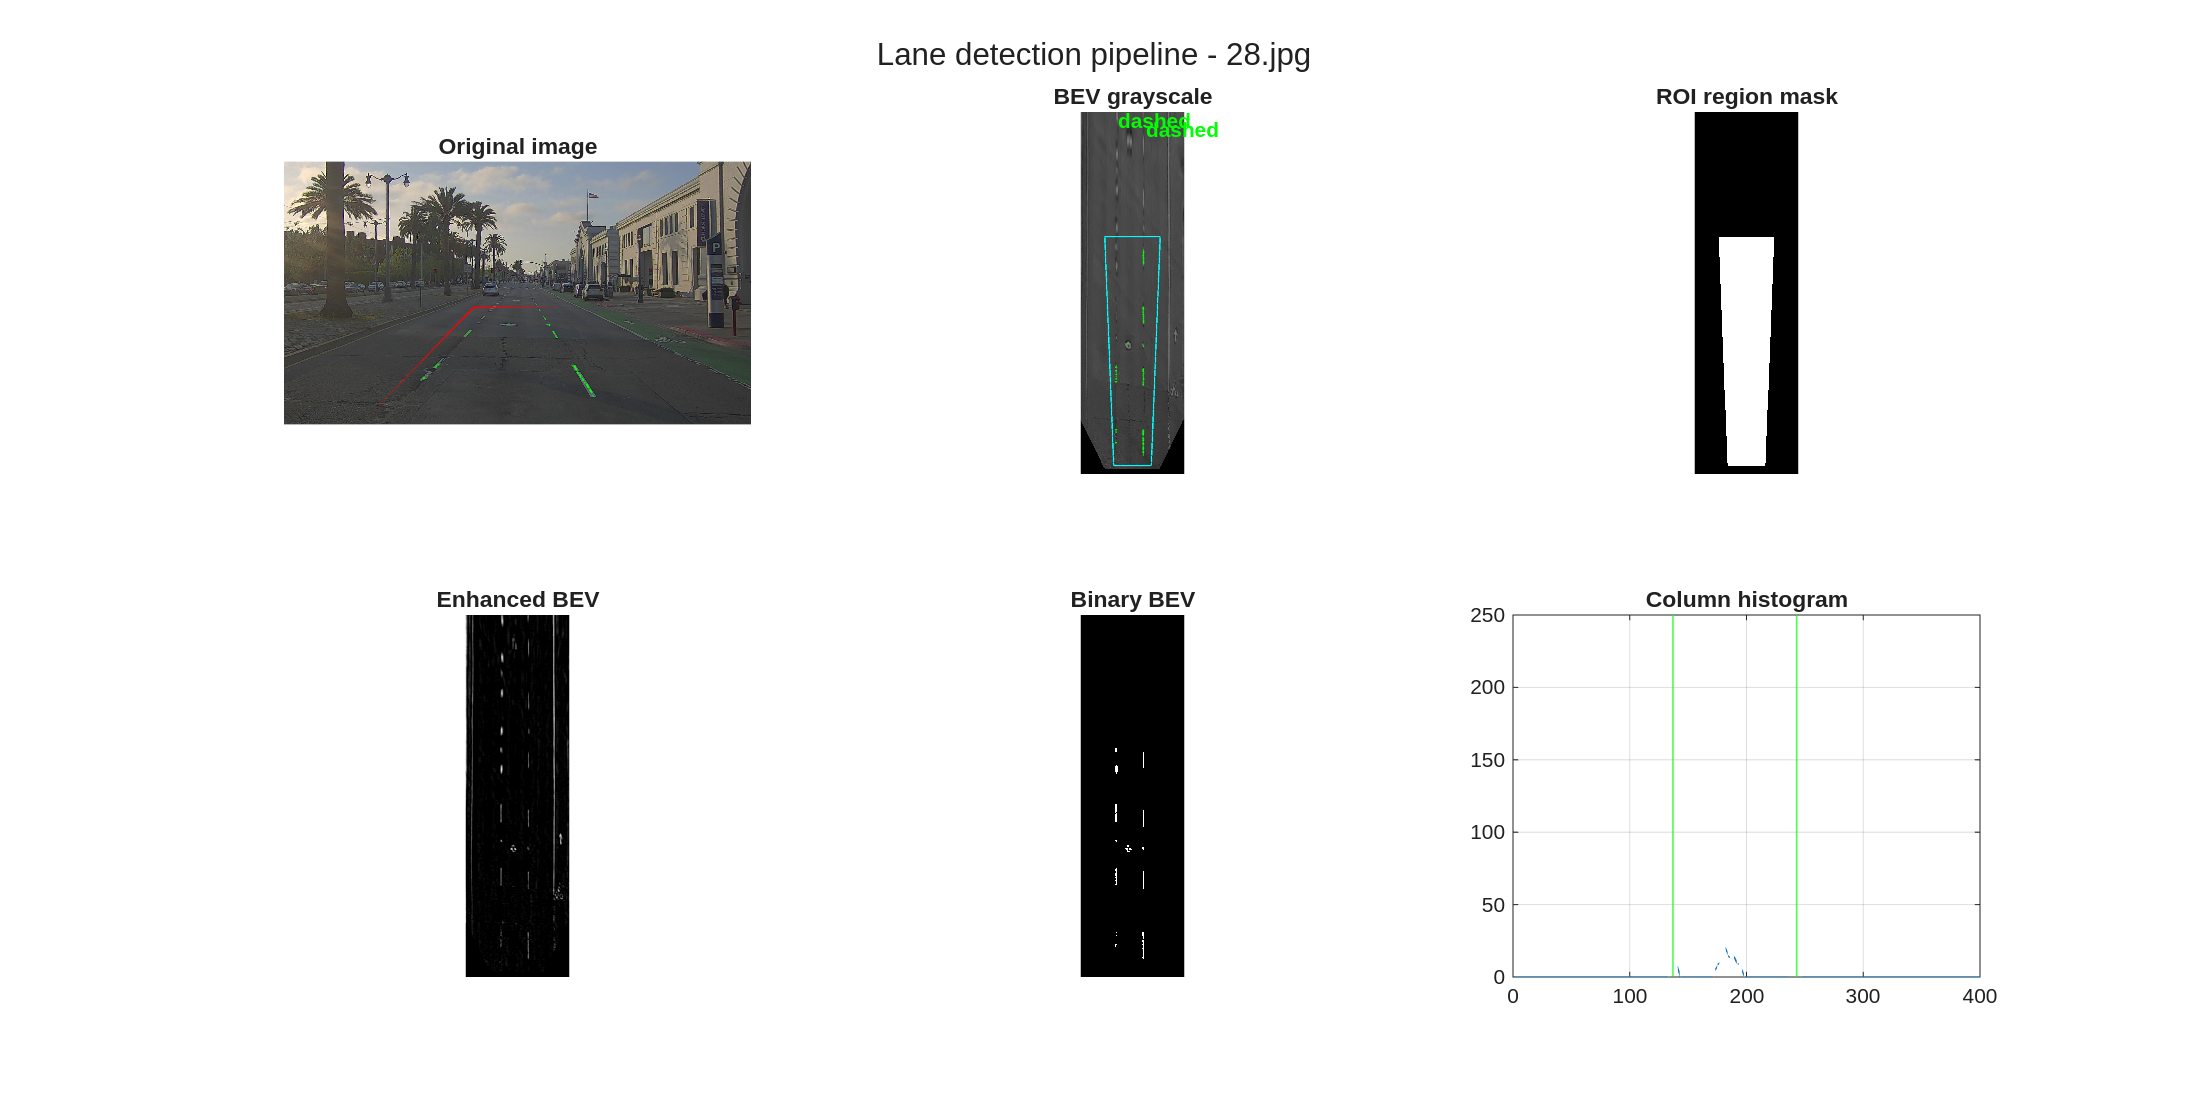
\includegraphics[width=0.5\textwidth]{images/21_result_dash.png}
    \caption{Scenario 21: dashed lane detection with road-surface noise.}
    \label{scenario21}
\end{figure}

Scenario 21 was used as a first validation case for the lane-marking pipeline. As shown in Fig.~\ref{scenario21}, the method correctly identifies the visible lane boundaries and classifies the markings as dashed. Some local noise is still visible in the intermediate binary image and in the histogram, mainly due to road texture and manholes, but the peak-based initialization and the row-wise tracing are sufficiently robust to preserve the final lane estimate.


\begin{figure}[htbp]
    \centering
    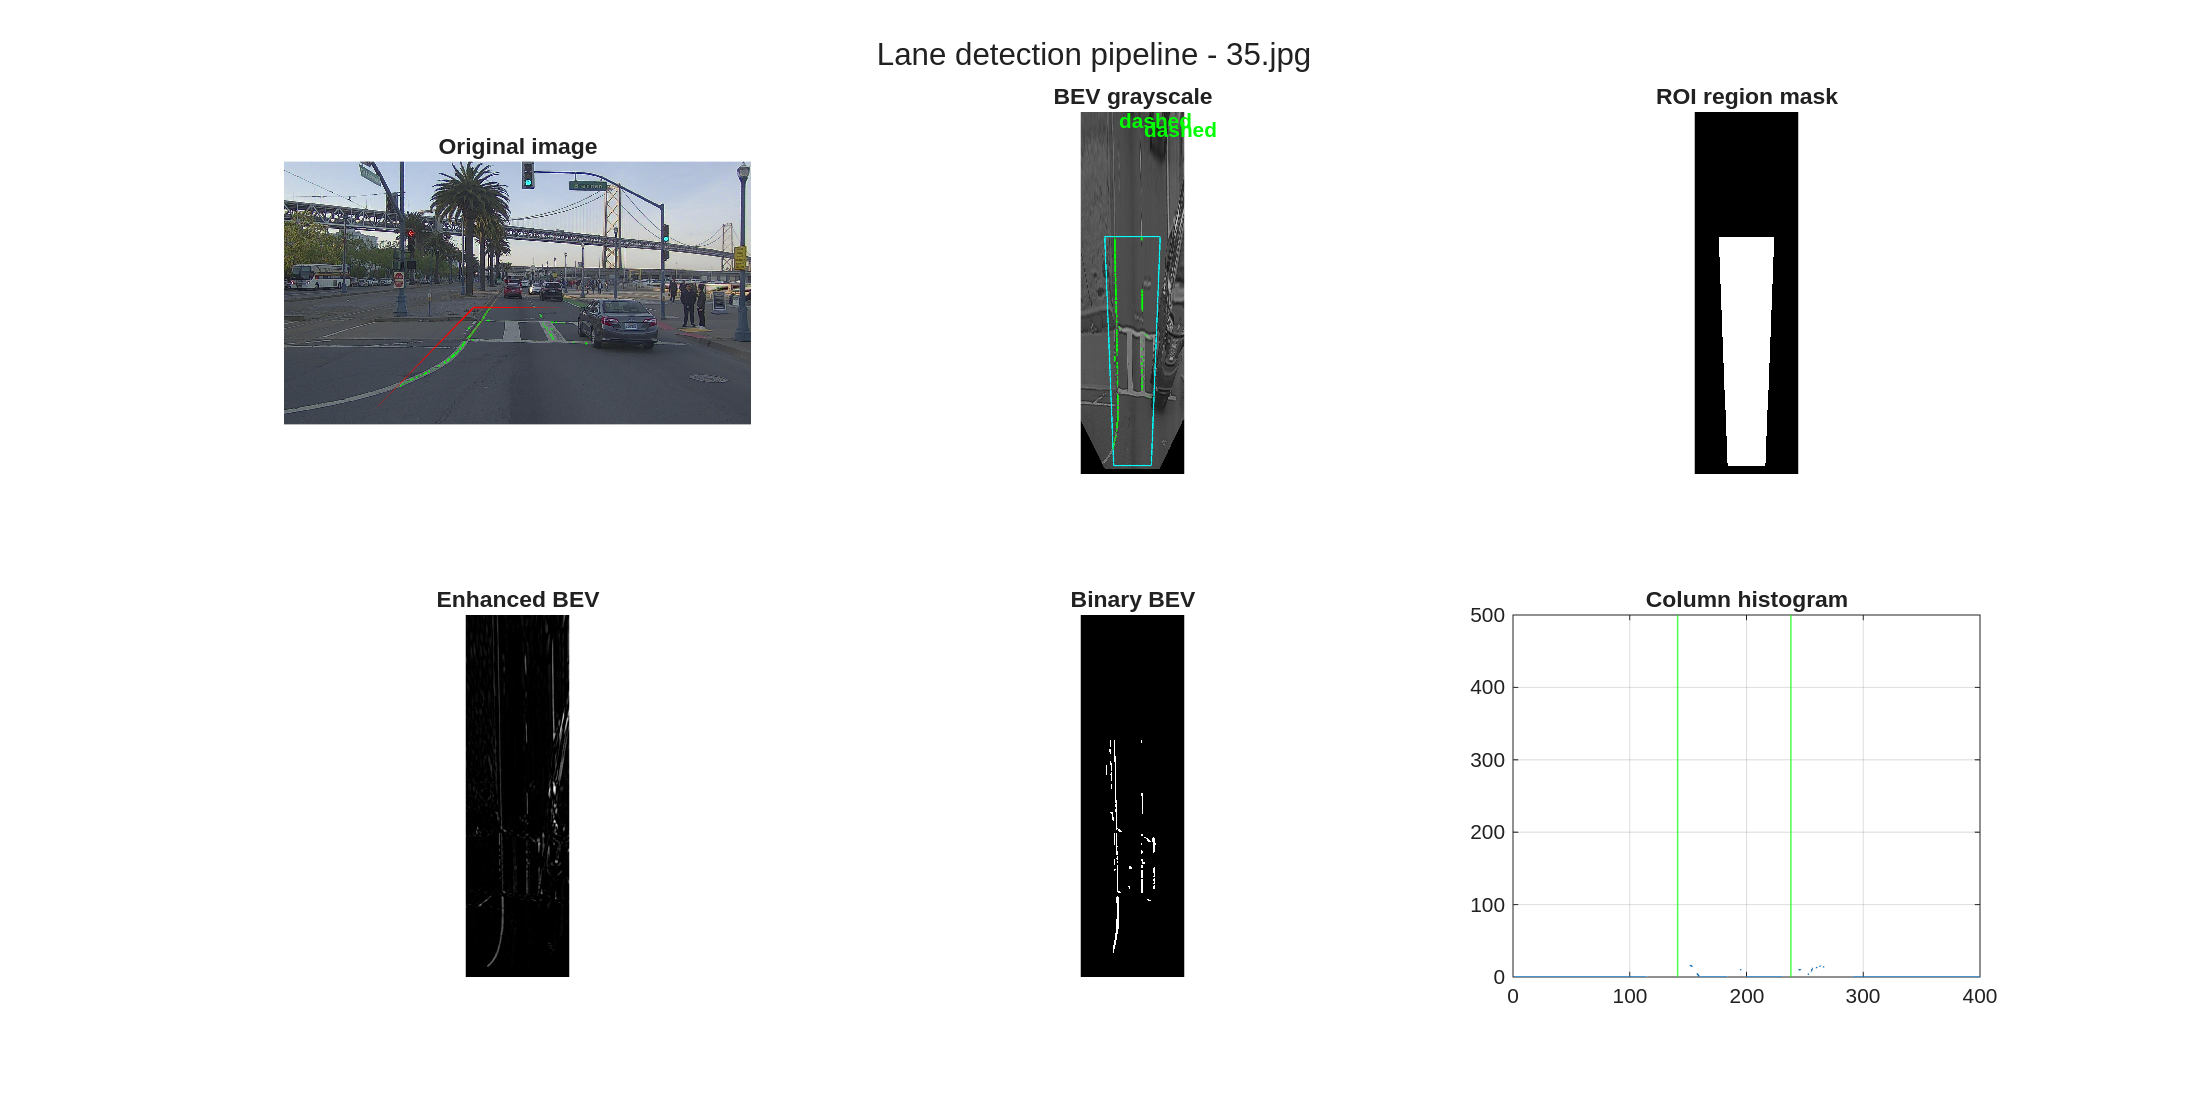
\includegraphics[width=0.5\textwidth]{images/11_result_dash.png}
    \caption{Scenario 11: curved dashed markings near an intersection.}
    \label{scenario11}
\end{figure}

Scenario 11 (Fig. \ref{scenario11}) highlights the advantage of tracing the lane row by row instead of drawing only vertical lines in BEV. In this sequence, the dashed markings are curved and describe the boundaries of an intersection area. The output shows that the algorithm is still able to follow the curved dashed structure and to project it back onto the original camera image with a coherent geometry.

Scenario 46 (Fig. \ref{scenario46}) provides a more challenging case because the presence of a road user partially occludes the road region. The obstacle mask removes the corresponding area from the valid ROI used for lane extraction, reducing the risk that the object texture is interpreted as a lane marking. This behaviour is visible in the ROI mask and confirms that obstacle information can also support the lane-detection stage by suppressing potentially misleading pixels.
\begin{figure}[htbp]
    \centering
    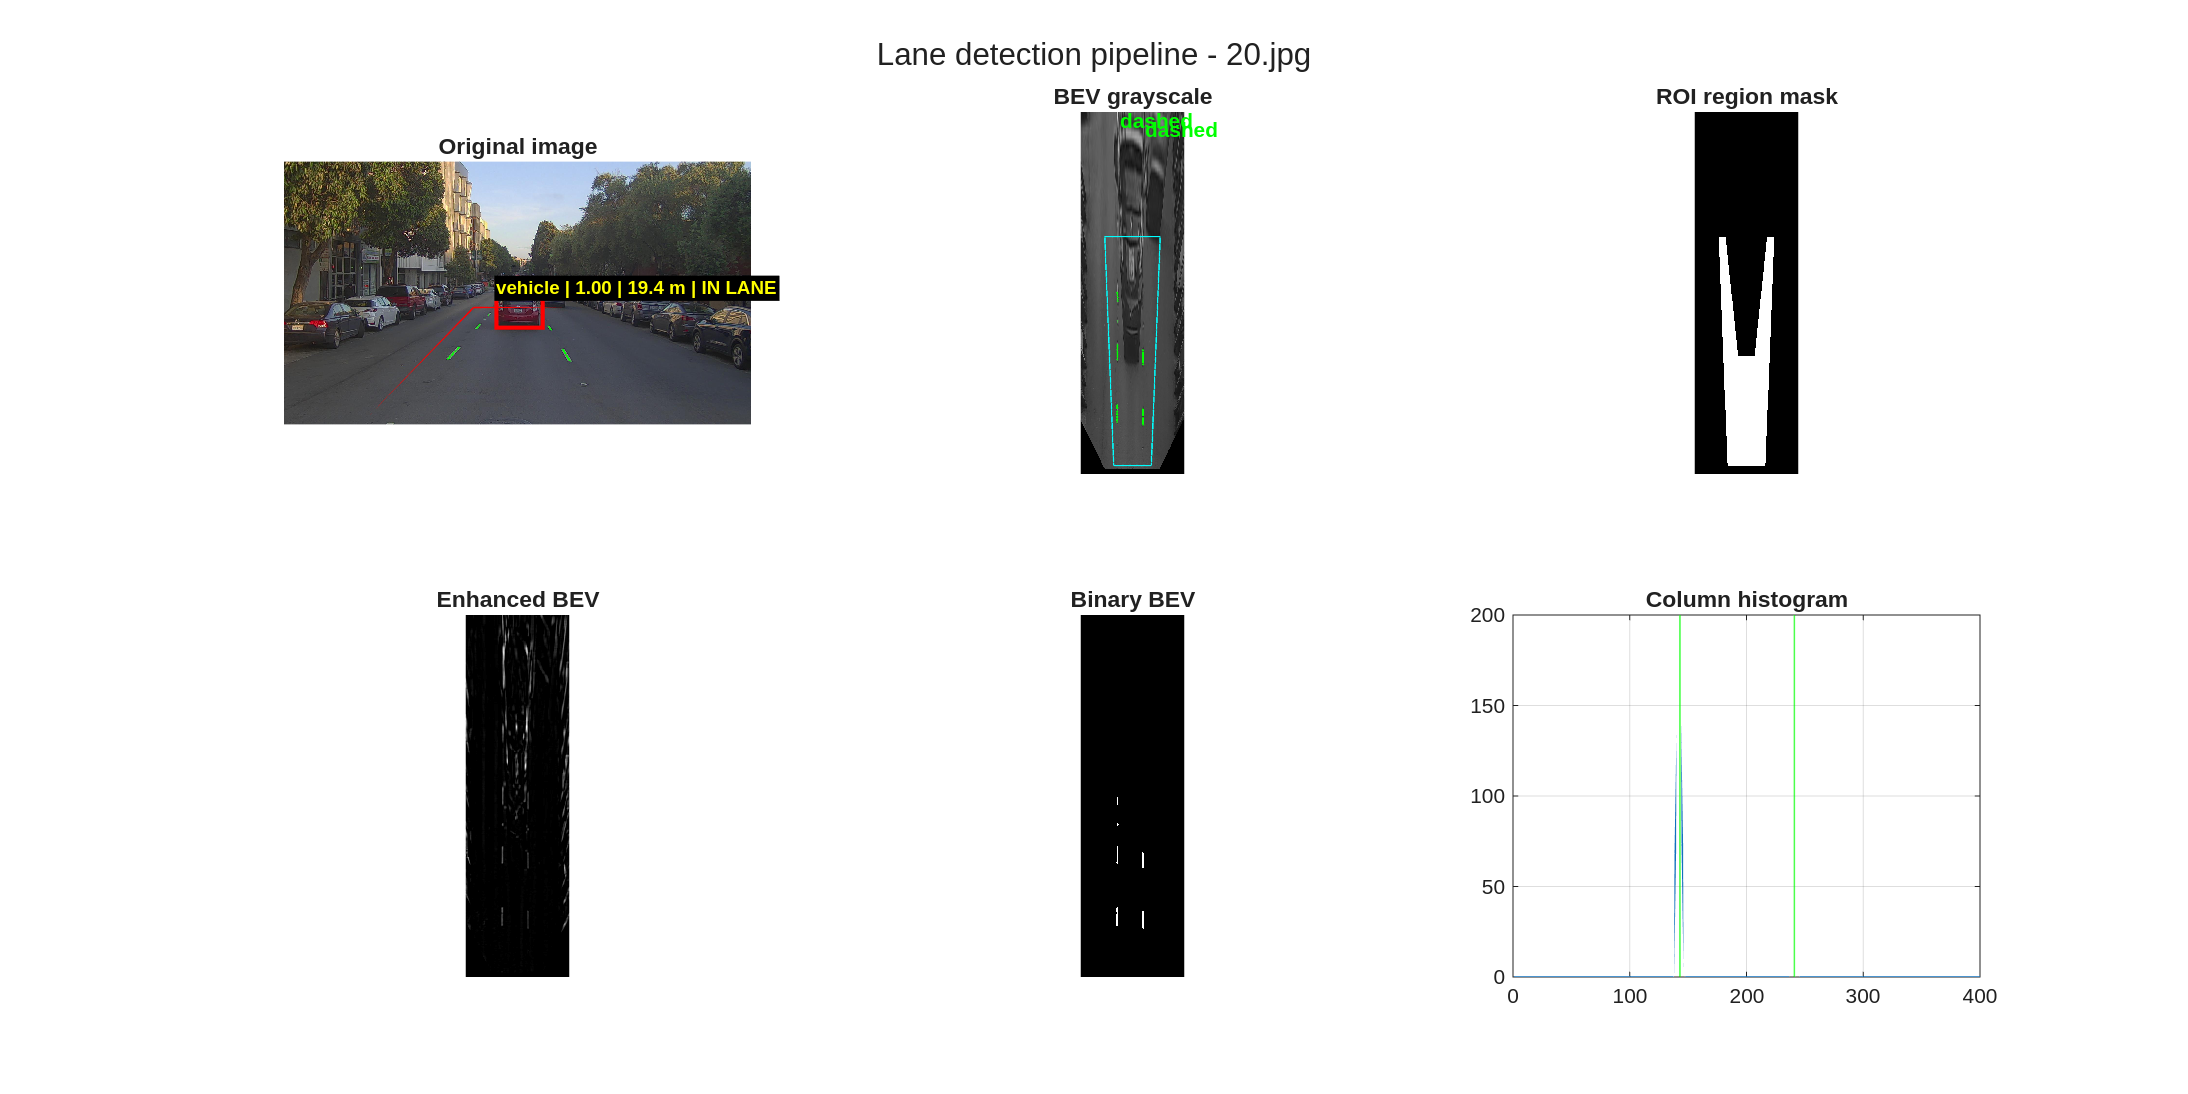
\includegraphics[width=0.5\textwidth]{images/46_result_dash.png}
    \caption{Scenario 46: obstacle-aware ROI masking}
    \label{scenario46}
\end{figure}

The obstacle-detection extension was tested mainly on scenarios 44 (Fig. \ref{scenario44}) and 2 (Fig. \ref{scenario2}), where traffic participants are clearly visible in the camera view. In scenario 44, the detector identifies road users while the lane pipeline continues to operate across a change in road slope, from an uphill portion to a downhill portion. This indicates that the BEV-based processing remains usable even when the apparent road geometry changes along the sequence.

\begin{figure}[htbp]
    \centering
    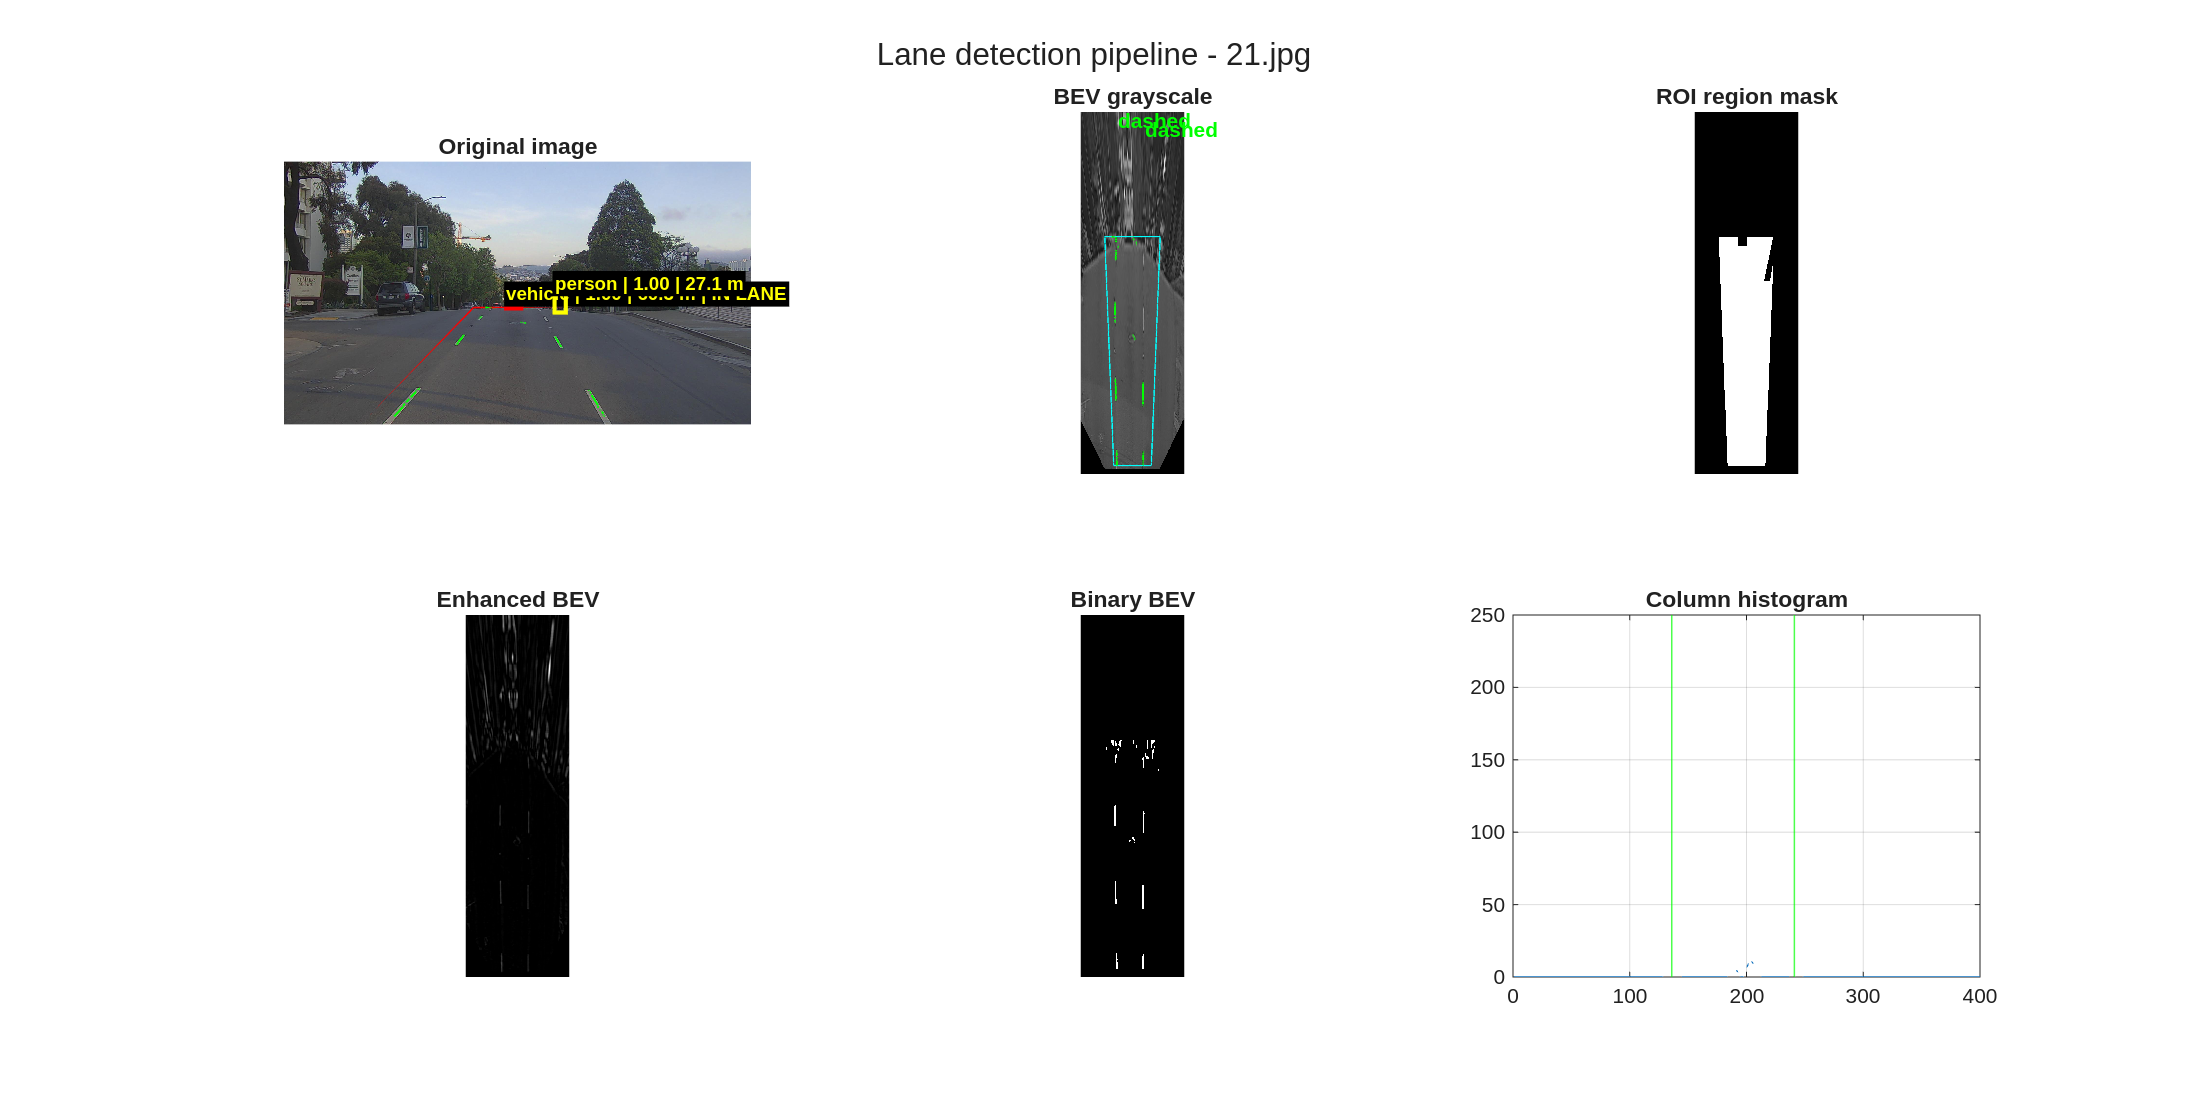
\includegraphics[width=0.5\textwidth]{images/44_result_obj.png}
    \caption{Scenario 44: road-user detection together with lane estimation.}
    \label{scenario44}
\end{figure}

Scenario 2 contains vehicles that are much closer to the ego vehicle. In these frames, the bounding boxes make the obstacle-detection output visually explicit and the colour coding highlights detections that are estimated to lie inside the current driving lane. The approximate distance label provides an additional cue for interpreting the scene, even though it remains a coarse estimate based only on bounding-box height.

\begin{figure}[htbp]
    \centering
    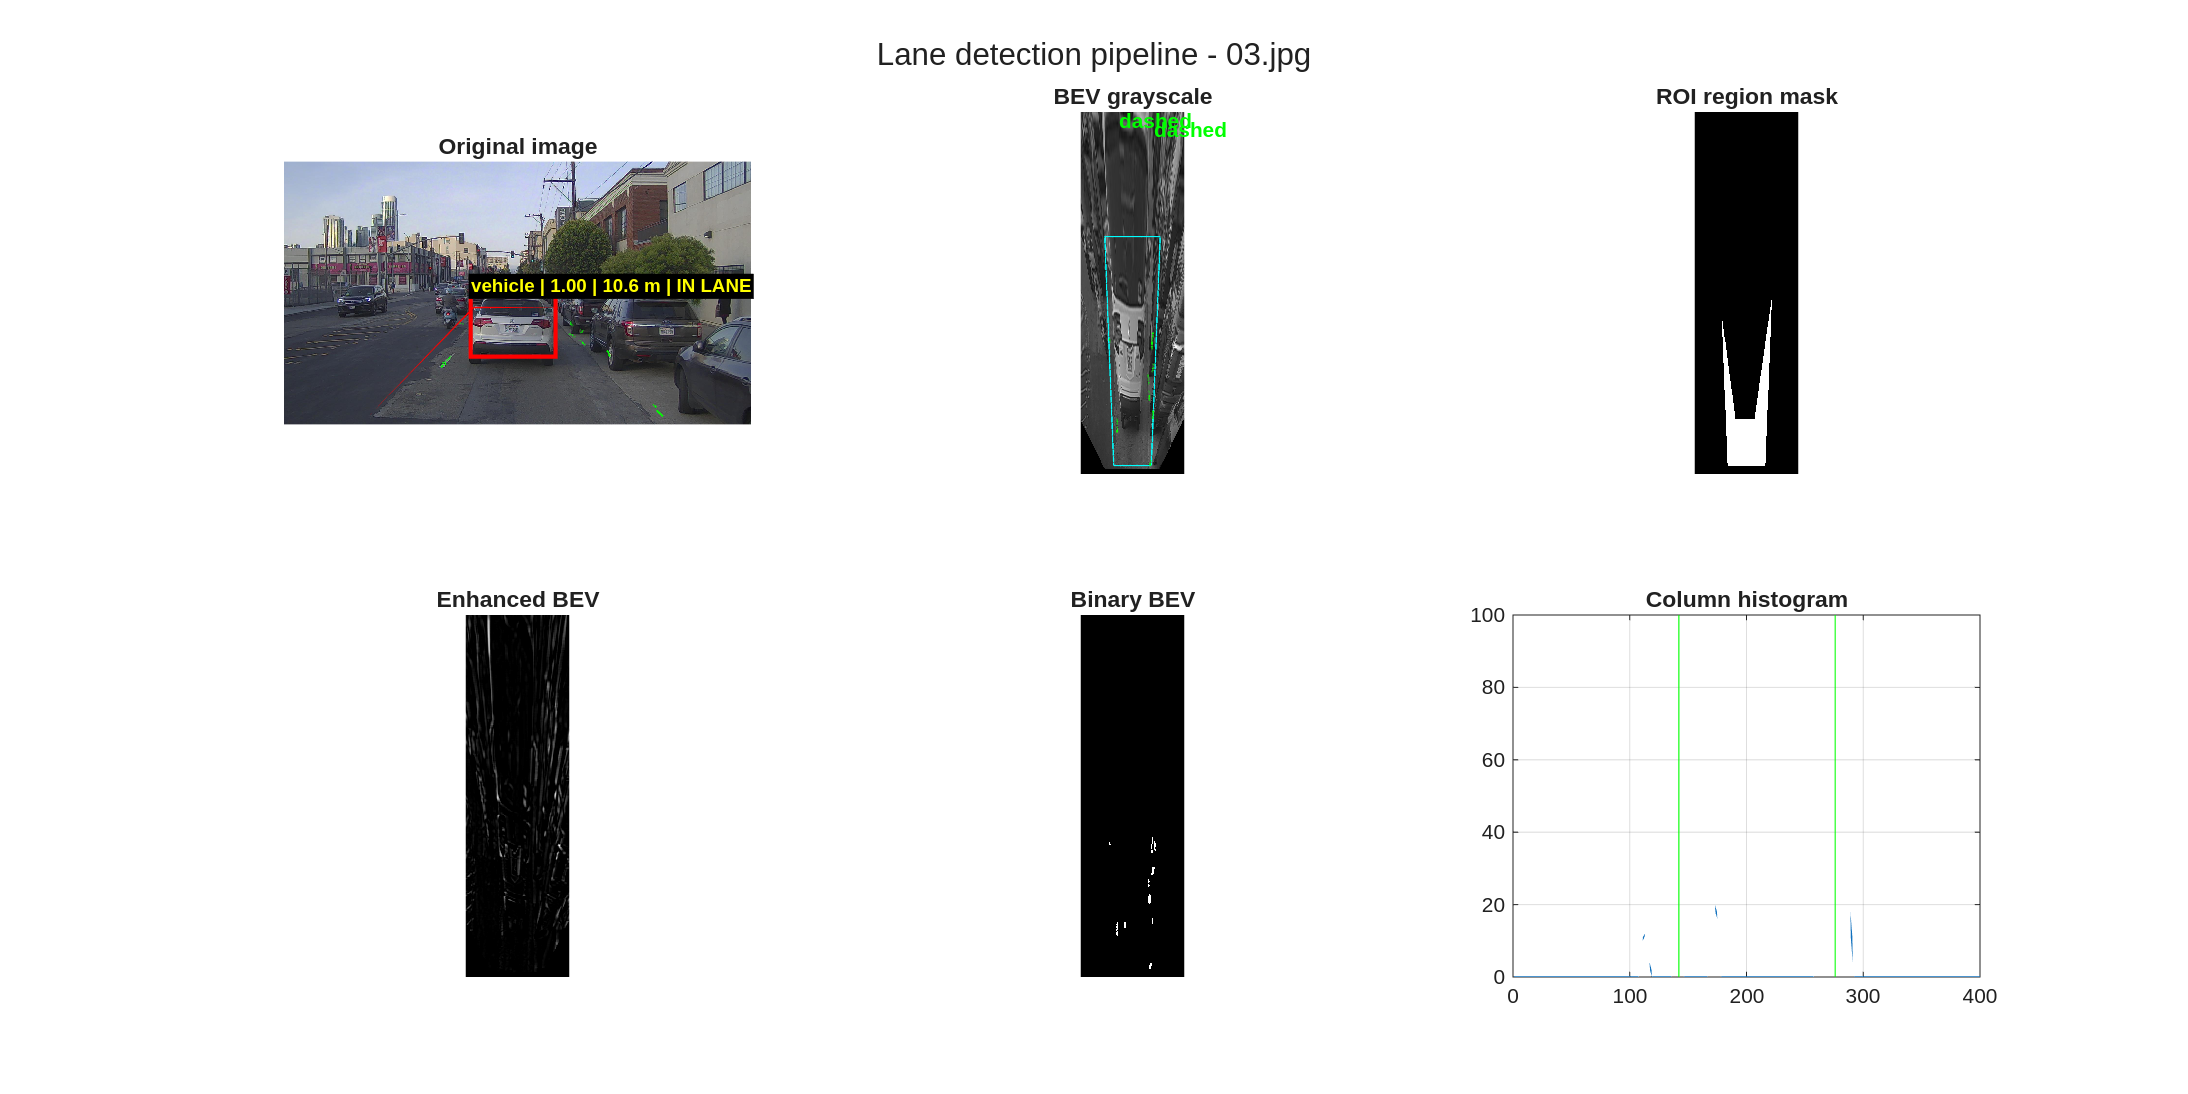
\includegraphics[width=0.5\textwidth]{images/2_result_obj.png}
    \caption{Scenario 2: close vehicles and distance-aware visualization.}
    \label{scenario2}
\end{figure}


\section{Conclusion}

This report presented a MATLAB implementation of a lane detection pipeline inspired by the GOLD methodology and extended with obstacle detection. The proposed solution combines geometric reasoning, classical image processing, and object detection to address both the mandatory and optional requirements of the assignment.

The experimental results show that the pipeline is able to detect both straight and curved lane markings, project the estimated lanes back onto the original image, and integrate obstacle detections within the driving lane. The use of a Bird’s Eye View representation, together with histogram-based initialization and row-wise tracking, proved effective for handling moderate road curvature and varying lane appearances.

However, the qualitative evaluation also highlighted some limitations. The main sources of error are related to strong illumination changes, worn or partially occluded lane markings, and noise in the binarized BEV image, which directly affects the histogram-based initialization. These observations indicate that the overall robustness of the system is strongly dependent on the quality of the binary segmentation stage.

Future work could focus on improving the stability of the preprocessing stage, for instance through more robust road-surface filtering, refined connected-component analysis, or the introduction of a more advanced temporal model for lane and obstacle tracking.


\bibliographystyle{IEEEtran}
\bibliography{reference}

\vspace{8pt}
\acknowledgments{A public repository is available online at \href{https://github.com/annamaroma/Technologies4AutonomousVehicles}{\textit{this}} link and includes the folder \textit{Assignment2} with the Matlab scripts useful to complete the exercises.}

\end{document}
